\documentclass{ecai}
\usepackage{times}
\usepackage{graphicx}
\usepackage{latexsym}
\usepackage{xspace}
\usepackage{hyperref}
\usepackage{amssymb}
\usepackage{algorithm}
\usepackage[noend]{algpseudocode}
\usepackage[numbers]{natbib}
\usepackage{notoccite}
\usepackage{framed}
\usepackage{amsmath}
\usepackage{tabularx}

\usepackage[dvipsnames]{xcolor}
\newcommand{\sergey}[1]{\textcolor{magenta}{{\sc Sergey:} #1}\xspace}
\newcommand{\samuel}[1]{\textcolor{green}{{\sc Samuel:} #1}\xspace}
\newcommand{\tias}[1]{\textcolor{blue}{{\sc Tias:} #1}\xspace}

\newcommand{\constraints}{\ensuremath{\mathcal{T}}\xspace}
\newcommand{\format}[1]{\textit{#1}\xspace}
\newcommand{\generategroups}{\format{generateAssignments}}
\newcommand{\extractgroups}{\format{extractGroups}}
\newcommand{\extracttables}{\format{extractTables}}
\newcommand{\learnconstraints}{\format{learnConstraints}}
\newcommand{\findassignment}{\format{findSolutions}}
\newcommand{\postprocess}{\format{pruneRedundant}}
\newcommand{\constrainttorder}{\format{generalityOrder}}
\newcommand{\template}{\format{Constraint template}}


\newcommand{\CName}{Name\xspace}
\newcommand{\CSignature}{Signature\xspace}
\newcommand{\CFunction}{Function\xspace}
\newcommand{\dependencies}{\ensuremath{\mathcal{D}}\xspace}
\newcommand{\groups}{\ensuremath{\mathcal{G}}\xspace}

\newcommand{\range}[3]{\ensuremath{#1[#2,#3]}}
\newcommand{\rangeto}[2]{#1{:}#2}
\newcommand{\rangeall}{:}

\newcommand{\eccalc}[2]{\ensuremath{#1 = #2}}
\newcommand{\ecrank}[2]{\eccalc{#1}{\mathit{RANK}(#2)}}
\newcommand{\ecfkey}[2]{\ensuremath{#1 \rightarrow #2}}
\newcommand{\ecalldiff}[1]{\ensuremath{\mathit{ALLDIFFERENT}(#1)}}
\newcommand{\eclookupf}[4]{\ensuremath{\mathit{LOOKUP}_{#4}(#1, #2, #3)}}
\newcommand{\eclookup}[4]{\eccalc{#1}{\eclookupf{#2}{#3}{#4}{}}}
\newcommand{\eclookupprod}[5]{\eccalc{#1}{#2 \times \eclookupf{#3}{#4}{#5}{}}}
\newcommand{\eclookupfuzzy}[4]{\eccalc{#1}{\eclookupf{#2}{#3}{#4}{fuzzy}}}
\newcommand{\ecperm}[1]{\ensuremath{\mathit{PERMUTATION}(#1)}}
\newcommand{\ecseries}[1]{\ensuremath{\mathit{SERIES}(#1)}}
\newcommand{\ecprod}[3]{\eccalc{#1}{#2 \times #3}}
\newcommand{\ectotal}[3]{\eccalc{#1}{\mathit{PREV}(#1) + #2 - #3}}
\newcommand{\ecproj}[2]{\eccalc{#1}{\mathit{PROJECT}(#2)}}
\newcommand{\ecaggc}[3]{\eccalc{#2}{\mathit{#1}(#3, col)}}
\newcommand{\ecaggr}[3]{\eccalc{#2}{\mathit{#1}(#3, row)}}
\newcommand{\ecsumc}[2]{\eccalc{#1}{\mathit{SUM}(#2, col)}}
\newcommand{\ecsumr}[2]{\eccalc{#1}{\mathit{SUM}(#2, row)}}
\newcommand{\ecaggif}[5]{\eccalc{#2}{\mathit{#1IF}(#3, #4, #5)}}
\newcommand{\ecsumif}[4]{\eccalc{#1}{\mathit{SUMIF}(#2, #3, #4)}}
\newcommand{\ecsumprod}[3]{\eccalc{#1}{\mathit{SUMPRODUCT}(#2, #3)}}

\newcommand{\luc}[1]{{\textcolor{red}{#1}}}





%%\ecaisubmission   % inserts page numbers. Use only for submission of paper.
                  % Do NOT use for camera-ready version of paper.

\begin{document}

\title{Tabular Constraint Learning}

\author{Name1 Surname1 \and Name2 Surname2 \and Name3 Surname3 \institute{KU Leuven, Belgium, email: firstname.lastname@kuleuven} }

\maketitle

\begin{abstract}
  abstract
\end{abstract}

\section{Introduction}
Millions of people across the world use spreadsheets everyday.
Yet, many people lack a complete understanding of the structures and existing dependencies in the data.
Indeed, the most useful part of spreadsheets is often the formulas and often these formula disappear when a file is exported and shared, for example as a CSV file.
This brings us to the question: can we discover or reconstruct structural relations in flat tabular spreadsheet data?
Moreover, can we accomplish this task in a general way that allows declarative specification of constraints to discover?


Let us look at an example in Figure~\ref{fig:main_example}, the header names already suggest the usage of standard spreadsheet operations such as \textit{average} or \textit{sum}.
If we look at Table~1 and at the first row in Table~2, it is clear that one could have selected the column called \textbf{1st Quarter}, clicked on the \textit{SUM} function and then just used the drag fill handle to apply the formula to the other columns.
Similarly, that would work for the second (\textit{Average}), third (\textit{Min})  and forth (\textit{Max}) rows in Table 2.
I.e., all operations are vectorized and make use of the standard spreadsheet operations.

Examining Table~1 also shows that computations are not only performed column-wise but row-wise as well: the cells in the column \textbf{Total} are obtained by taking the row-wise sum of the previous four columns.

That gives us already a hint how this problem is different from the standard data mining settings, when the data is in rows and variables are in columns. Here everything is mixed, some values are missing in the results, some missing the arguments, even a header might have missing values. The data is relational on one hand, since we have multiple table with relationships between them. And on the other hand, the data is numeric, since people tend to use spreadsheets for financial and accounting computations, which is heavily numeric.

Given these novel aspects, we conclude that understanding and learning constraints in tabular data is a new and challenging problem setting.
Futhermore, it is not only challenging for a machine but for a human as well.

Due to the complexity of numeric computations in spreadsheets, people often fail to grasp the properties of the data, which leads to so called the Spreadsheet risk\footnote{\url{https://en.wikipedia.org/wiki/Spreadsheet\#Spreadsheet_risk}} and even caused major flaw in the famous economics papers \cite{flaw_excel} and caused billion-losses in the financial industry \cite{spreadsheet_risk_loss}. Tabular constraint learning provides a potential cure by indicating learned constraint violations and suggest possible fixes.

\sergey{bullet points for Luc and Tias to rework introduction}\\
\textbf{Motivation}:
\samuel{Suggest better table layouts / formula translation}
\begin{itemize}
  \item File generated from model, model got lost, need to reconstruct
  \item Constraint programming is hard - is Excel hard?
  \item Avoid manual analysis, provide selection of constraints
  \item Error checking
  \item Completion, gain speed and insights (Complicated constraints, also complicated to verify, too much output)
\end{itemize}

\textbf{Novelty:}
\begin{itemize}
  \item Unsupervised setting (contrary to flashfill, etc)
  \item Numeric, different constraints (contrary to single textual function solution in flashfill, etc)
  \item Data format (2D) -- data is no longer in rows like a classic ML or DM settings
  \item Declarative, general / modular, stacking of constraint problems
\end{itemize}

\sergey{need to elaborate the example here: like in a story}

\begin{figure*}[tbh]
  \begin{center}
    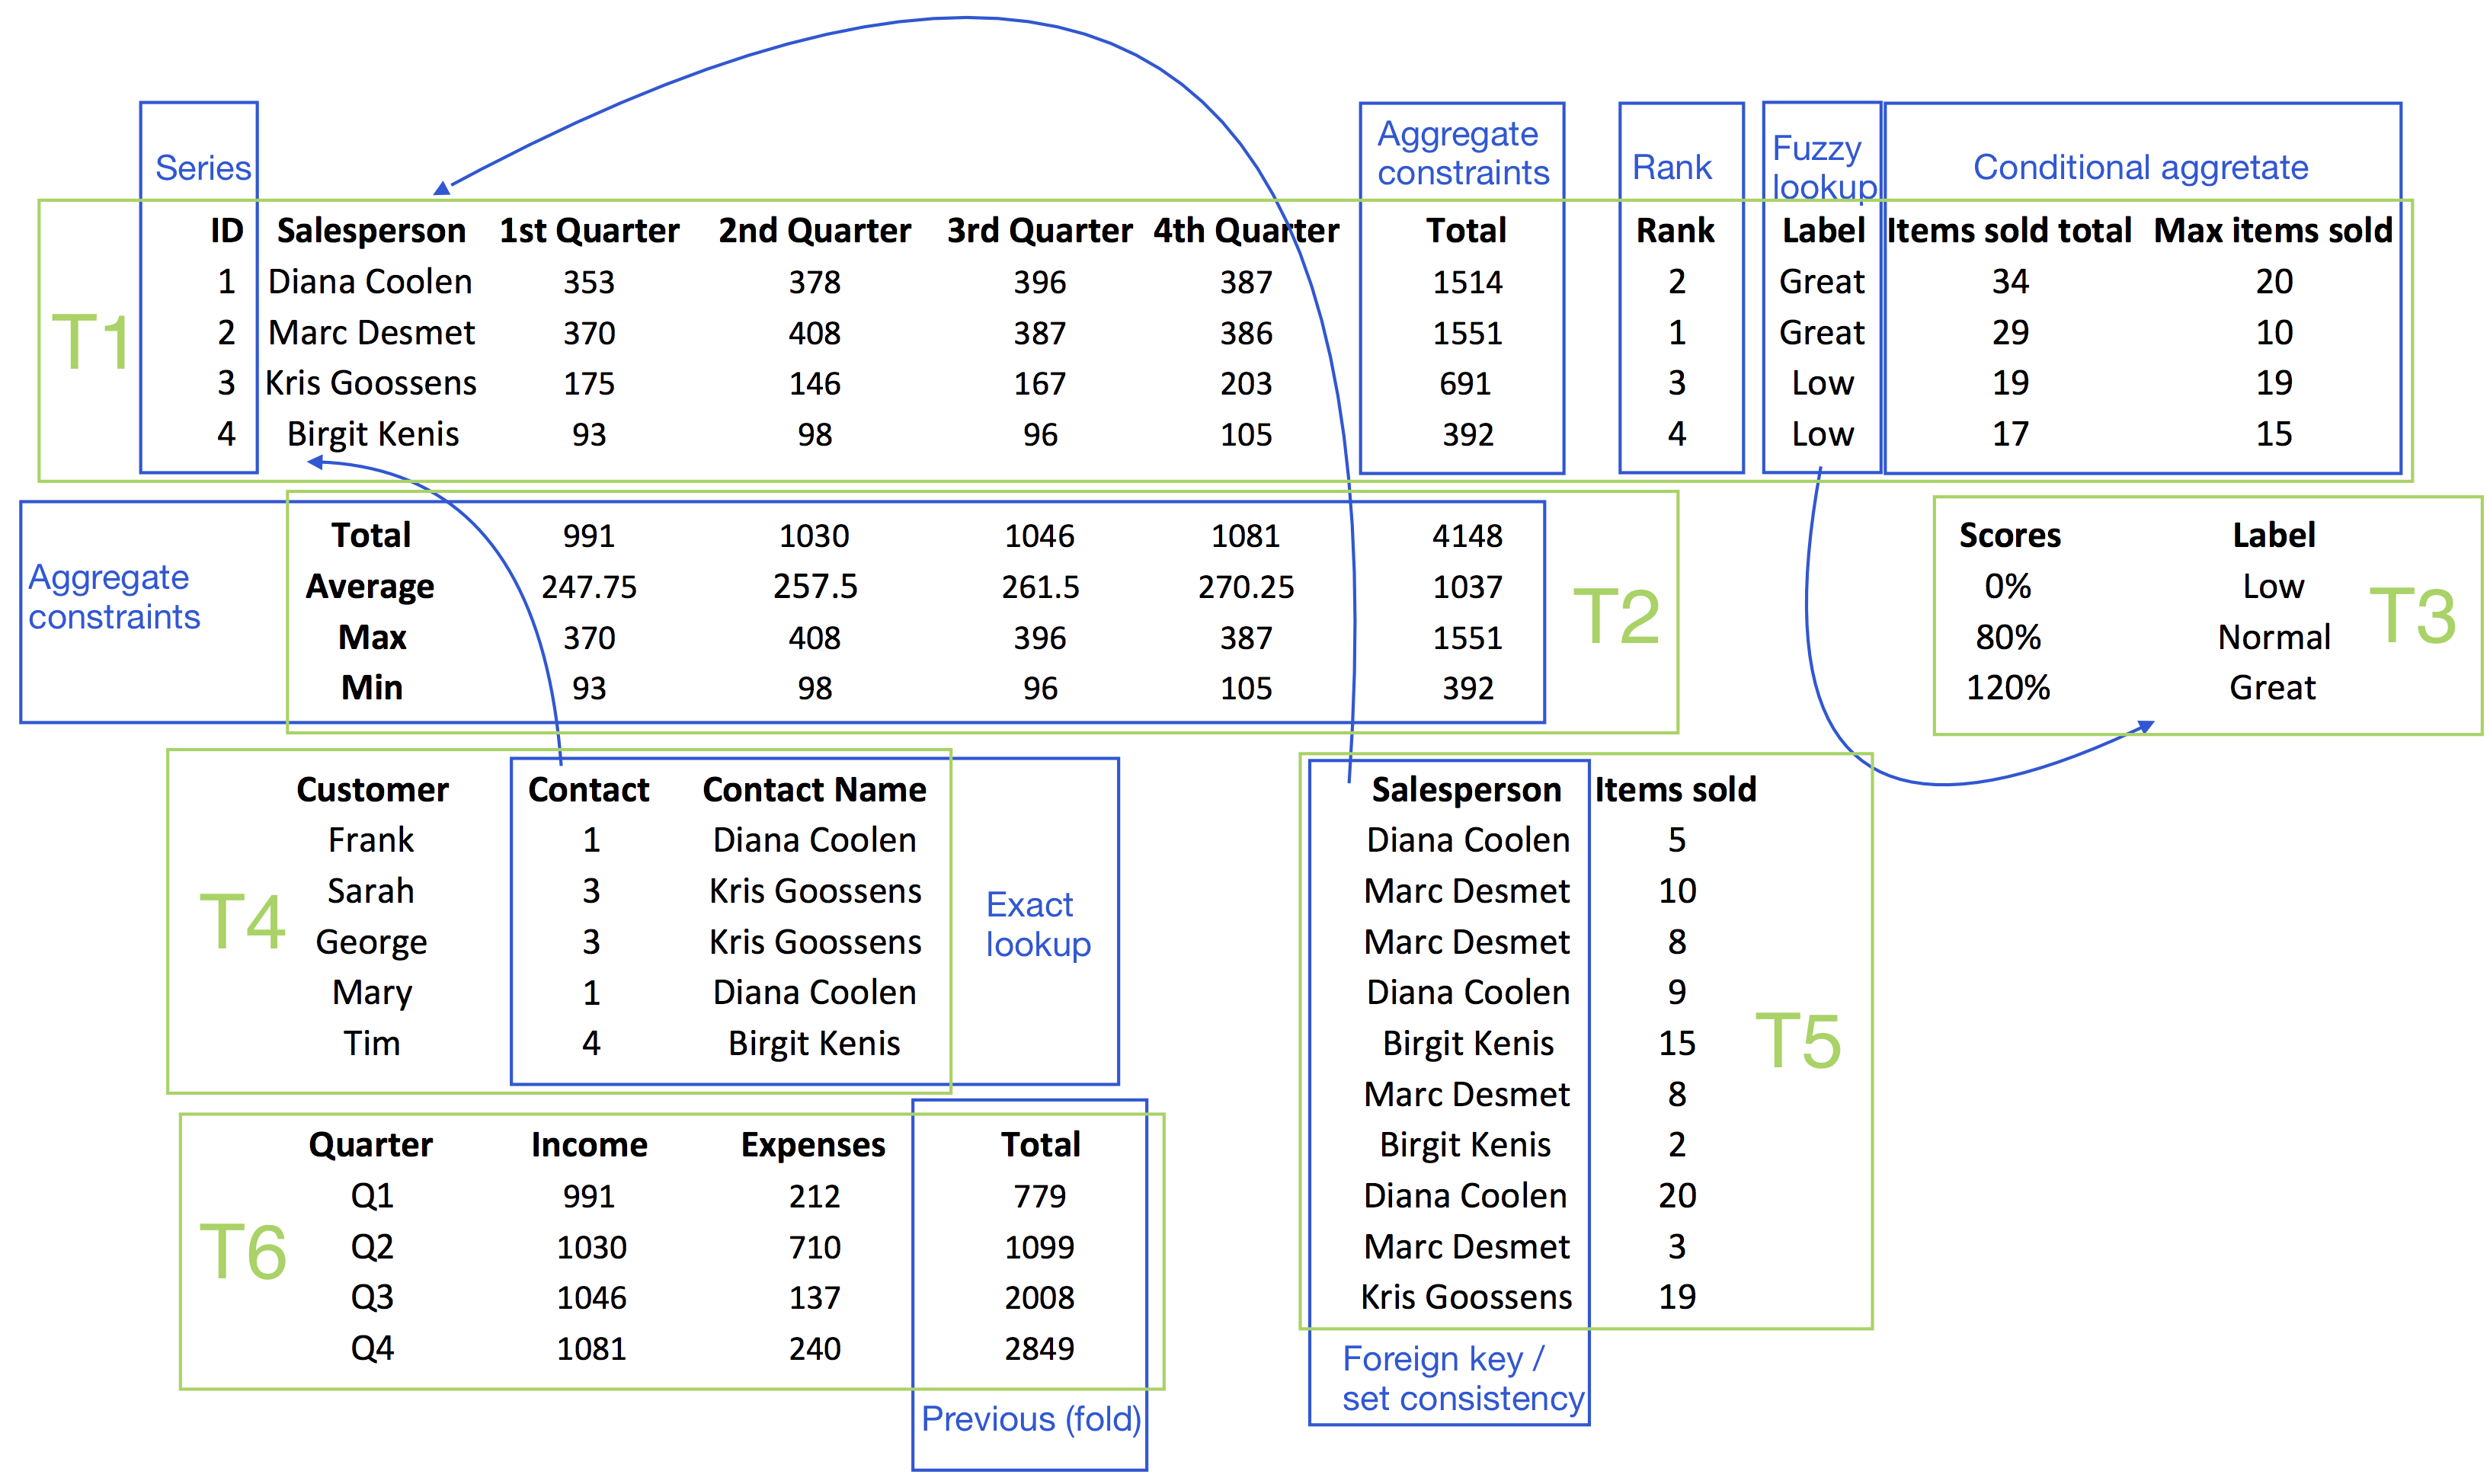
\includegraphics[width=0.75\textwidth]{figures/Demo.png}
  \end{center}
  \vspace{-10pt}
  \caption{An example of constraint reconstruction (in blue) with indicated groups (in green)}
  \label{fig:main_example}
\end{figure*}

\section{Formalization}
\samuel{Explain concepts on example}
\sergey{subgroup notation, rework the solution definition}
\subsection{Groups, Type-consistency and Constraints}
In this work we focus on spreadsheet data, which is physically one big table, but conceptually often consists of multiple tables, see Figure~\ref{fig:main_example} for an example.
Formally, a table is an $n \times m$ matrix, each table entry is called  a \textit{cell}.

Each cell has a {\em type} which can be numeric or textual.
The numeric type has two subtypes: integers and floats.
We also consider the special element called \textit{None}, which can be either type: numeric or textual.
A set of cells is called \textit{type-consistent} iff all cells in the set are either numeric or textual.
%Certain constraints, such as \textit{rank} or \textit{series}, make use of the numeric subtype by requiring its arguments to be integers.

We consider various sets of cells in tables:
\begin{itemize}
  \item {\bf Cells}: Each entry in the matrix/table is called  a \textit{cell}.
  We use the notation $T[a,b]$ to refer to a particular cell in the table~$T$ at the row with index~$a$ and the column with index~$b$.
  \item {\bf Columns and rows}: To refer to the $a$-th row (column) we use the following syntax $T[a,{:}]$ ($T[{:},a]$), to refer to a subrange from $a$ to $b$ we use $T[a{:}b,]$ ($T[,a{:}b]$).
  \item
  A \textit{vector} is either a column or a row that is type-consistent.
  If a vector is a row (column), we say that it has a \textit{row} (\textit{column}) orientation.
  \item
  A \textit{group} is a subrange of vectors with the same orientation in a table.
  We use the following notation to refer to a row (column) group $G$ in a table $T$ with rows (columns) ranging from $a$ to $b$: $G = T[a{:}b,:]$ ($G = T[{:},a{:}b]$), where $a,b$ are natural numbers.
  We denote as the \textit{length} of a row (column) group $G$, written as \textit{length(G)}, the number of its columns (rows). We call a group $G$ \textit{numeric} (\textit{textual}, etc), written as \textit{numeric(G)}, if all its vectors contain numeric (textual, etc) elements.
  \item
 A \textit{subgroup} $g$ is a subrange of vectors belonging to a group $G$. If the subgroup $g$ must contain only one vector, we write $g \in G$. It defines what it means for a constraint to be well-formed
%We refer to a subgroup of a group $G$ in \groups as $g$. A \textit{subgroup} $g$ is a subrange of vectors in a group $G$. If a subgroup $g$ must contain only one vector, we write $g \in G$.
% A \textit{subgroup} $G'$ is a subrange of vectors belonging to a group $G$. If the subgroup $\{v\}$ must contain only one vector, we write $v \in G$.
\end{itemize}
For notational convenience, we will refer to vectors with $V$ and to groups and subgroups with $G$.

When we do not want to distinguish between cells, columns, rows, vectors or groups, we shall talk about a {\em set of cells}.

\paragraph{Example}
Consider Table~1 in the Figure~\ref{fig:main_example}, its rows are not type consistent (i.e. they contain both numeric and textual data).
The (column) vectors of Table~1 are subdivided into five groups:
\begin{align*}
&G_1 = \range{T_1}{\rangeall}{1},
&G_2 = \range{T_1}{\rangeall}{2},\\
&G_3 = \range{T_1}{\rangeall}{\rangeto{3}{8}},
&G_4 = \range{T_1}{\rangeall}{9},\\
&G_5 = \range{T_1}{\rangeall}{\rangeto{10}{11}}.
\end{align*}
In order to sum the results of a salesperson across quarters we can consider for example the subgroup $\range{T_1}{\rangeall}{\rangeto{3}{6}} \subset G_3$

\subsection{Constraints}
A \template is a triple \textit{(\CName, \CSignature, \CFunction)}.
Let us elaborate on each of them. 
\begin{itemize}
\item
\textit{\CName} is the textual name of the constraint together with the list of its variables $v_1,\dots,v_n$.  In ILP terminology, it is known as vocabulary.
\item
  \textit{\CSignature} is a set of constraints on the properties of the group assignments, corresponding to the variables $v_1,\dots,v_n$ in \CName.
  For example, the signature can restrict the types of the groups, e.g., requiring them to be integers or constrain their sizes, e.g. the length of vectors in the arguments must be equal.
  The constraints act on properties or group meta-information, not on the actual group content. In ILP, it is known as bias, it defines what it means for a constraint be well-formed.
  \item \textit{\CFunction} is a constraint specifying that the data in the subgroups satisfies the function. In ILP, it is known as background knowledge, which provides a definition to a predicate.
\end{itemize}

\paragraph{Example}
  For example, the \template \textit{rank} has
\begin{itemize}
\item \CName: \textit{$v_r$ = RANK($v_x$)}, where $v_x$ and $v_r$ are its variables;
\item \CSignature: groups assigned to $v_x$ must be numeric, groups assigned to $v_y$ must be integer and the length of vectors in $v_x$ is the same as in $v_y$;
\item \CFunction: the mapping $\{ v_x \mapsto g_x, v_y \mapsto g_y \}$ satisfies the constraint iff $g_x \in G_x, g_y \in G_y$ ($G_x \in \groups, G_y \in \groups$) and each value in $g_y$ is the rank of the corresponding value in $g_x$ (possibly with ties).
\end{itemize}


\section{Problem Statement}
\sergey{moved from the formalization BEGIN}
We can now define a classical constraint satisfaction problem on tables.
A {\em constraint satisfaction problem} (CSP)  consists of 1) a set of cells, and 2) a set of constraints over those cells.
Notice that the constraints specify the types (or the domains) that one encounters in traditional CSPs.
Notice also, that as in traditional CSPs, the CSP problem defines the variables (the cells) of the problem as well as the constraint that should hold amongst them. The task of CSP-solvers is then to find an assignment to the variables that satisfies all the constraints.
The distinction between variables (cells) and their assignments (their values) is important here.
So, when we speak about cells, vectors and groups, we refer to the variables; when we talk about values, assignments or instances, we refer to the values these cells take in a particular "instantiated" table.

While the traditional CSP problem is given a set of cells and a set of constraints,
and the task is to find an assignment, the {\bf inverse CSP} or the {\bf Tabular Constraint Learning Problem} can be defined as follows.\\
\\
{\bf Given }
\begin{itemize}
\item
a set of instantiated tables (so all cells have values) ${\cal T}$;
\item
a set of \template ${\cal C}$;
\item
a set of groups ${\cal G}$ for the tables ${\cal T}$;
\end{itemize}
\noindent
\samuel{This section is incorrect, yet, we find assignments over subgroups, associated with a \template}
{\bf Find}  the set $C\subseteq {\cal C}$ that contains all constraints $c(G_1, ... , G_N)$ that 1) are satisfied  in ${\cal T}$, 2)
for which
all $G_i \in {\cal G}$ and  3)  $c(G_1, ... , G_N)$ satisfies the signature of the constraint $c$.


\luc{ADD/REFER TO EXAMPLE}

Let us introduce \template instantiation syntax. Let $S$ be a mapping from variables to the subgroups of \groups and $t$ be a \template, then $t^S$ is the template, in which all variables in all constrainst in \CSignature and \CFunction are instantiated with the corresponding subgroups from $S$. We refer to $t^S$ as a \textit{constraint} and to the instantiated \CSignature (\CFunction) as $\text{\CSignature}^S$ ($\text{\CFunction}^S$). Throughout the work we refer as \textit{find constraints} to finding all constraints that hold.


Let us now define what it means for a constraint from \template to hold in general. Let $t$ be a \template, $S$ be a mapping from variables to the subgroups of \groups, and $C$ be the constraint $t^S$, then $C$ \textit{holds} iff all constraints in $\text{\CSignature}^S$ and $\text{\CFunction}^S$ of $C$ hold.
\sergey{moved from formalization END}

In the previous section we introduced the problem of tabular constraint learning informally using the example in Figure \ref{fig:main_example}. Here we formalize the statement in terms of \template and group assignments as follows: 

\begin{minipage}[c]{14em}
  \vspace{5pt}
  \begin{tabular}{ll}
    \multicolumn{2}{l}{{\textbf{Tabular Constraint Learning Problem}}}\\
    \vspace{-4pt}
    &\\
    \textbf{Given:}& the set of all groups $\groups$ and of \template $\constraints$\\
    \textbf{Find:}&  all constraints $C$ over \groups for each template $t$ in \constraints \\
  \end{tabular}
  \vspace{6pt}
\end{minipage}

  The key observation here is that essentially the problem is a constraint enumeration problem, where each constraint is independent. This property comes from fact that in spreadsheets each formula is applied based on the existing data in the cells. This allows learning constraints independently of each other by examining constraint satisfaction on the groups.


  In theory each constraint is independent and equally useful. In practice, however, things are different. Assume that for some $g_x$ both \textit{series($g_x$)} and \textit{alldifferent($g_x$)} hold. From a user's perspective the last solution is useless, since he or she already knows that the series constraint implies the alldifferent constraint. To capture this condensed representation \cite{condensed} of solutions, we have introduced a specificity (generality) order between constraints, which is depicted using solid (dashed) arrows in Figure \ref{fig:learning_order}. This matters from implementation perspective as well, if we discovered that $g_x$ is not a permutation, then $g_x$ should not be tested for the series constraint at all. A solid lines from $t_1$ to $t_2$ indicates that $t_2$ is \textit{more specific} than $t_1$ and if $C_1=t_1^S$ from $t_1$ does not hold, then the constraint $C_2=t_2^S$ from $t_2$ does not hold neither. A dashed arrow from $t_1$ to $t_2$ indicates that $t_1$ is \textit{a more specific} constraint than $t_2$ and therefore if $C=t_1^S$ from $t_1$ holds it should not be tested for $t_2$.


Let $t$ be a \template, $S$ be a mapping from variables to the subgroups of \groups, \dependencies be the DAG of constraint specificity, then the constraint $C$ equal to $t^S$ is called  \textit{the most specific} wrt \dependencies iff $C$ holds and there is no other template $t_{*}$ for which the constraint $C_{*}=t_{*}^S$ holds and $t_{*}$ is more specific in \dependencies.


Let us introduce the version of tabular constraint learning that takes into account the specificity relation between constraints.

\begin{minipage}[c]{14em}
  \vspace{5pt}
  \begin{tabular}{ll}
    \multicolumn{2}{l}{{\textbf{Condensed Tabular Constraint Learning Problem}}}\\
    \vspace{-4pt}
    &\\
    \textbf{Given:}& the set of all groups $\groups$ and of \template's $\constraints$,\\
    & a constraint specificity DAG \dependencies \\
    \textbf{Find:}& all the most specific wrt \dependencies constraints $C$ over \groups\\
    & for each $t$ in \constraints \\
  \end{tabular}
  \vspace{6pt}
\end{minipage}

This version explicitly takes into account the specificity of the constraints and invalidates some of the solutions that are entailed by the tabular other solutions.

\section{Approach to Tabular Constraint Learning}
\sergey{Luc wants this to be more intuitive, should we just add some examples here to make it easier to follow and refer to the running example?}
As we have seen in the statement before we assume the set of groups to be given. It is often, however, not the case and a possible approach is to extract the groups from the CSV file directly. In our system, we have implemented the group construction step using the type-consistency check. \sergey{Samuel, we need details here, I think} In general, separating data from a header is a task on its own  \cite{header} and goes beyond the scope of this paper.

Another solution to the group extraction problem is to make it interactive, when a user can select the groups in the spreadsheet or correct automatically generated groups. We regard this approach to be a possible future direction in the system development. Later in the paper we assume the groups to be given.

Now we describe how the problem of Condensed Tabular Constraint Learning can be solved. The algorithm mimics the structure of the problem in the following way: first we need to order constraints in the order of specificity, then for each constraint we need to generate possible candidate groups, and in the next step we find the subgroups satisfying the constraint. After an iteration we accumulate all solutions and proceed to the next constraint.

\begin{algorithm}[thb]
  \begin{algorithmic}
    \footnotesize
    \State \textbf{Input:} $\groups$ -- groups, $\constraints$ -- \template's, \dependencies -- dependency graph
    \State \textbf{Output:} $C$ -- learned constraints 
    \State $C \gets \emptyset$ \Comment{The set of constraints}
  \For{$t \in \constrainttorder(\constraints,\dependencies)$}
  \State $v_1, ..., v_n =$ variables of $T$
    \For{$v_1{:}~G_1, \dots, v_n{:}~G_n \in \generategroups(t, \groups, C, \dependencies)$}
      \State $C \gets C \cup \findassignment(t, v_1{:}~G_1, \dots, v_n{:}~G_n, C, \dependencies)$
    \EndFor
  \EndFor\\
\Return $C$
\end{algorithmic}
\caption{Tabular constraint learning}
\label{algo:tcl}
\end{algorithm}
Essentially, our Algorithm \ref{algo:tcl} has three steps: constraint ordering, candidate group generation and subgroup satisfaction search, which is in line with the ``generate-and-test'' paradigm that is well-known in AI \cite{whaisasp}. Let us elaborate on each step in detail.

\samuel{Running example (RANK?)}

\subsection{Constraint ordering} 
Since some constraints are more general than the other, we generate them in the generality order similar to the ILP techniques known as refinement operators \cite{luc_book}.

$\constrainttorder(\constraints,\dependencies)$ uses the DAG~\dependencies in Figure \ref{fig:learning_order} in the following way: all constraints are generated in the topological order of~\dependencies.
Solid edges point from more general to more specific constraints.
Therefore, if there is a solid edge from constraint~$t_1$ to constraint~$t_2$, then a set of subgroups satisfying~$t_2$ must contain the subgroups satisfying~$t_1$.

Dashed edges represent the inverse relationship, pointing from specific to more general constraints.
If there is a dashed edge from $t_1$ to $t_2$, then a set of subgroups satisfying $t_2$ may not contain a subset that also satisfies $t_1$.

Thus, \dependencies describes a partial order in which constraints should be learned.
Some constraints have no dependencies (omitted from the figure) and can be learned independently.
Generally, a parallel version of the algorithm could learn each connected component independently, only taking into account the partial ordering within components.

\paragraph{Example}
\samuel{Fix notation variable vs. group}
Consider the \ecfkey{v_{fk}}{v_{pk}} (foreign-key) constraint: for every solution the subgroup (vector) $V$ assigned to $\mathit{v_{pk}}$ must fulfill \ecalldiff{V}.
Therefore, we say indicate \textit{foreign-key} as being dependent on \textit{all-different} and the latter will be treated first.
The \ecrank{v_y}{v_x} constraint does not have any dependencies, however in a restricted version without ties the vector $v_y$ would always be a permutation of numbers $1, 2, ..., \textit{length}(v_y)$.

\subsection{Candidate group generation}
$\generategroups(\textit{Constraint,GroupSet,Solutions})$ is the function generating tuples of groups that may contains subgroups satisfying the constraint.
The goal of this step is to prune out impossible groups from the beginning by looking at their properties rather than their actual content (\CSignature vs \CFunction).

Finding candidate groups for a \template~$t$ can be seen as a Constraint Satisfaction Problem (CSP) dependent on the \CSignature of $t$.
Several constraints (e.g. sum, max, count) have the same candidate generation procedure as they share the same \CSignature.

\paragraph{Example}
The \ecrank{v_y}{v_x} constraint requires $v_y$ to consist of only integer or only textual data and $v_x$ to be numeric.
This allows us to filter candidate groups for these variables.
Additionally, $v_y$ and~$v_x$ must be vectors of the same length, therefore, only groups with the same length are considered.
Groups that do not satisfy these requirements cannot contain subgroups (vectors) that satisfy \ecrank{v_y}{v_x}.

\subsection{Subgroup satisfaction search}
$\findassignment(\textit{Constraint,Candidates,Solutions})$ is the function that searches for subsets of vectors in the candidate groups that satisfy the constraint.
Every \template~$t$ needs to have an implementation that finds subgroup assignments, given set of tuples each containing a candidate group for every variable in~$t$.

\paragraph{Example}
Consider a candidate assignment $G_x, G_y$ associated with the variables $v_x,v_y$ of \ecrank{v_y}{v_x}, then \findassignment selects single vectors $g_y \in G_y, g_x \in G_x$ such that \ecrank{g_y}{g_x} is true, i.e. it searches for a mapping $S$ where $v_x$ ($v_y$) must be mapped to a subgroup of $G_x$ ($G_y$).
For example, in Figure~\ref{fig:main_example} the group $G = \range{T_1}{\rangeall}{\rangeto{3}{8}}$ can serve as both $G_x$ and $G_y$.
Then \findassignment could select $g_x$ to be $\range{T_1}{\rangeall}{7}$ and $g_y$ to be $\range{T_1}{\rangeall}{8}$ which forms a valid solution.
\\\\
For some constraints (most notably aggregates) there may be multiple overlapping subsets of a given group~$G$ that satisfy the constraint.
We chose to omit subsets that are fully contained within a larger subset since this can lead to overfitting.
If the returned subsets are too large and accidentally contain unrelated vectors, the user can split such a group, disallowing.

\subsection{Implementation note} Essentially for each \template both \generategroups and \findassignment are separate constraint satisfaction problems. Hence, it is natural to solve them using declarative solvers. Even though each is a separate constraint problem, they are variations of each other and can be modeled using similar techniques. It also makes an extension of the system easy, we can solve new variations by adding, removing or modifying constraints from a similar constraint satisfaction problem. Furthermore, declarative languages such as ASP \cite{whaisasp} and Minizinc \cite{minizinc} provide primitives that make modeling transparent and generic.

Our system internally supports ASP (using Clingo 4.5.4 \cite{clingo}), Minizinc (Gecode-backend 2.0.2 \cite{minizinc}) and a native Python CSP solver \cite{python_constraint}. All the constraints mentioned in the paper can be run purely using the internal Python engine without any external software. Future versions of the system will provide user interfaces to the ASP, Minizinc and Python-Constraint languages to allow users to add new constraints in a declarative way.

\subsection{Constraints}

\begin{figure}[htb]
  \centering
  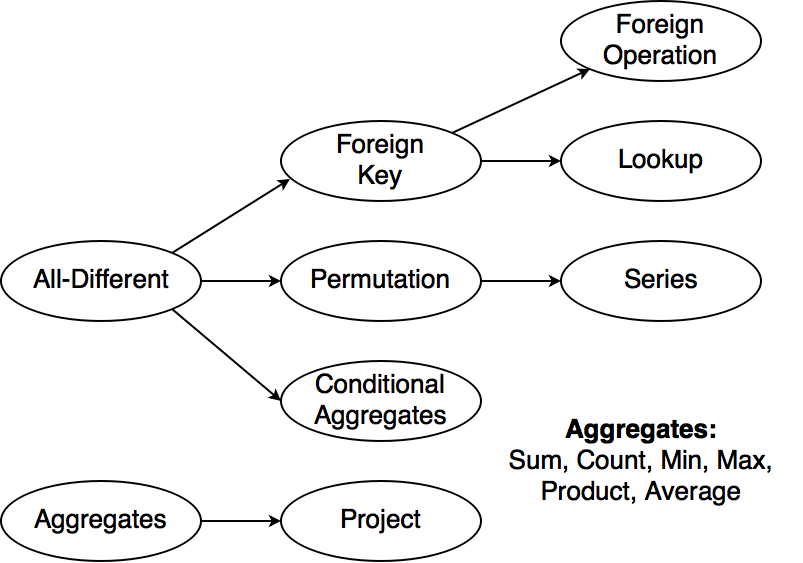
\includegraphics[width=0.20\textwidth]{figures/constraint_dependency.png}
  \caption{Constraint Learning Order. The solid arrows indicate a specificity order, i.e., \textit{permutation} $\rightarrow$ \textit{series} means that the series constraint is more specific than permutation. The dashed arrows indicate an inverse construction order, \textit{project} $\dashrightarrow$ \textit{aggregates} means the project constraint is more specific than aggregates. \sergey{Samuel,  can you give an explanation why we keep both arrow and how it is internally motivated?}}
  \label{fig:learning_order}
\end{figure}


\newcommand{\numeric}{\format{numeric}}
\newcommand{\textual}{\format{textual}}
\newcommand{\integer}{\format{integer}}
\newcommand{\discrete}{\format{discrete}}
\newcommand{\plength}{\format{length}}
\newcommand{\ptype}{\format{type}}
\newcommand{\ptable}{\format{table}}
\newcommand{\por}{\format{orientation}}
\newcommand{\prows}{\format{rows}}
\newcommand{\pcols}{\format{columns}}
\newcommand{\nat}{\mathcal{N}}

\sergey{Table should take into account our new notation and balance between formality and intuition, heh}
\begin{table*}
  \centering
  \begin{tabularx}{\textwidth}{l X X}
    \textbf{\CName} & \textbf{\CSignature} & \textbf{\CFunction}\\ \hline \hline
    \ecalldiff{v_x}
      & $\discrete(v_x)$
      & All values in $v_x$ are different: $v_x[i] \neq v_x[j]$ if $i \neq j$
      \\ \hline
    %X = Y & & \\
    \ecperm{v_x}
      & $\numeric(v_{x})$, $\ecalldiff{v_{x}}$
      & The values in $v_{x}$ are a permutation of the numbers $1$ through $\plength(v_{x})$.
      \\ \hline
    \ecseries{v_x}
      & $\numeric(v_{x})$ and $\ecperm{v_{x}}$
      & $v_{x}[1] = 1$ and $v_{x}[i] = v_{x}[i - 1] + 1$.
      \\ \hline
    \ecfkey{v_{fk}}{v_{pk}} & $v_{fk}$ and~$v_{pk}$ are both $\discrete$; $\ptype(v_{fk}) = \ptype(v_{pk})$; $\ptable(v_{fk}) \neq \ptable(v_{pk})$; and $\ecalldiff{v_{pk}}$ & Every value in~$v_{fk}$ also exist in~$v_{pk}$ \\ \hline
    % TODO check out
    \eclookup{v_r}{v_{fk}}{v_{pk}}{v_{val}}
      & $v_{fk}$ and $v_{pk}$ are both $\discrete$; variables $\{v_{fk}, v_{r}\}$ and $\{v_{pk}, v_{val}\}$ within the same set have the same \plength, \ptable and \por; $v_{r}$ and~$v_{val}$ have the same type; and \ecfkey{v_{fk}}{v_{pk}}.
      & $v_r[i]$ is the same value as looking up~$v_{fk}[i]$ in~$v_{pk}$  and returning the corresponding value in~$v_{val}$.
      \\ \hline
    \eclookupfuzzy{v_r}{v_{fk}}{v_{pk}}{v_{val}}
      & \textit{Same as lookup}
      & $v_r[i]$ is the same value as looking up the last item in~$v_{pk}$ smaller than~$v_{fk}[i]$ and returning the corresponding value in~$v_{val}$.
      \\ \hline
    \eclookupprod{v_r}{v_1}{v_{fk}}{v_{pk}}{v_{val}}
      & Variables $\{v_{r}, v_{1}, v_{fk}\}$ are $\numeric$, variables $\{v_{pk}, v_{val}\}$ are $\discrete$ and within both sets all variables have the same \plength, \ptable and \por; also \ecfkey{v_{fk}}{v_{pk}}.
      & $v_{r}[i]$ is the obtained by multiplying $v_{1}[i]$ with $\eclookupf{v_{fk}}{v_{pk}}{v_{val}}{}[i]$.
      \\ \hline
    \ecprod{v_r}{v_1}{v_2}
      & Variables $\{v_{r}, v_{1}, v_{2}\}$ are all $\numeric$ and have the same $\plength$
      & $v_{r}[i] = v_{1}[i] \times v_{2}[i]$.
      \\ \hline
    \ecproj{v_r}{\mathbf{v_x}}
      & Variables $\{v_{r}, \mathbf{v_x}\}$ all have the same $\plength$, $\por$, $\ptable$ and $\ptype$; $\mathbf{v_x}$ contains at least~2 vectors
      & At every position~$i$ in $1$ through $\plength(v_{r})$ there is exactly one vector~$v$ in $\mathbf{v_x}$ such that $v[i]$ is a non-blank value, then $v[i] = v_{r}[i]$.
      \\ \hline
    \ecrank{v_r}{v_x}
      & $\integer(v_{r})$; $\numeric(v_{x})$; and $\plength(v_{r}) = \plength(v_{x})$
      & The values in $v_{r}$ represent the rank (from largest to smallest) of the values in $v_{x}$ (including ties)
      \\ \hline
    \ectotal{v_r}{v_{pos}}{v_{neg}}
      & Variables $\{v_{r}, v_{pos}, v_{neg}\}$ are all $\numeric$ and all have the same $\plength$, which is at least $2$
      & The values in $v_{r}$ are a running total, each value $v_{r}[i] = v_{r}[i - 1] + v_{pos}[i] - v_{neg}[i]$.
      \\ \hline
    \ecsumc{v_r}{\mathbf{v_x}}
      & $v_r$ and $\mathbf{v_x}$ are $\numeric$; $\prows(\mathbf{v_x}) \geq 2$; and $\pcols(\mathbf{v_x}) = \plength(v_r)$
      & Each value in $v_{r}$ is obtained by summing over the corresponding column in $\mathbf{v_x}$.
      \\ \hline
    \ecsumr{v_r}{\mathbf{v_x}}
      & $v_r$ and $\mathbf{v_x}$ are $\numeric$; $\pcols(\mathbf{v_x}) \geq 2$; and $\prows(\mathbf{v_x}) = \plength(v_r)$
      & Each value in $v_{r}$ is obtained by summing over the corresponding row in $\mathbf{v_x}$.
      \\ \hline
    \ecsumif{v_r}{v_{fk}}{v_{pk}}{v_{val}}
      & $v_{fk}, v_{pk}$ are $\discrete$; $v_{r}, v_{val}$ are $\numeric$; within the sets $\{v_{val}, v_{fk}\}$ and $\{v_{pk}, v_{r}\}$ variables have the same $\plength$ and $\por$; $v_{fk}$ and $v_{val}$ have the same $\ptable$; $v_{fk}$ and $v_{pk}$ must have different $\ptable$s but the same $\ptype$; and \ecalldiff{v_{pk}}
      & The value for $v_{r}[i]$ is obtained by summing all values $v_{val}[j]$ where $v_{fk}[j] = v_{pk}[i]$
      \\ \hline
    \ecsumprod{v_r}{v_1}{v_2}
      & Variables $\{v_r, v_1, v_2\}$ are all $\numeric$; $\plength(v_{1}) = \plength(v_{2}) \geq 2$; and $\prows(v_{r}) = \pcols(v_{r}) = 1$
      & $v_{r}[i] = \sum_{i = 1}^{\plength(v_{1})} v_{1}[i] \times v_{2}[i]$.
      \\


  \end{tabularx}
  \caption{\template's \sergey{Here a detailed explanation on what is going on, what is essential, what is not? etc should be self-explanatory}\samuel{Motivate why product, not sum (=diff) you only need one, hardcoded preference for display} \sergey{1) should be readable alone without lookin in the text of the paper 2) that's the constraints we found popular according the spreadsheets in the web 3) that's what is actually implemented in the system 4) corresponds to the actual Excel functions}
} 
  \label{table:constraints}
\end{table*}

\samuel{Satisfy signature for group assignment: find groups such that there exists a subgroup which satisfies the signature}

% \subsection{Workflow}
% \begin{algorithm}[thb]
%   \begin{algorithmic}
%     \footnotesize
%     \State \textbf{Input:} $D$ -- dataset, \constraints -- constraints, \dependencies -- dependencies \\(optional: tables $T$, groups $G$)
%     \State \textbf{Output:} $S$ -- learned constraints with their satisfaction assignment
%     \If{$T$ is \textbf{not} provided}
%       \State $T \gets \extracttables(D)$
%     \EndIf
%     \If{$G$ is \textbf{not} provided}
%       \State $G \gets \extractgroups(D, T)$
%     \EndIf
%     \State $S \gets \learnconstraints(G,\constraints,\dependencies)$
%     \State \Return $S$
% \end{algorithmic}
% \caption{Workflow}
% \label{algo:workflow}
% \end{algorithm}

% \textbf{Approach}
% \begin{itemize}
%   \item Notation
%   \item Algorithm (select constraints, find assignments, find solutions)
% \end{itemize}

% \samuel{Move next to subgroup satisfaction search}
% \section{Declarative modeling}
% \sergey{We need to fit ASP, Minizinc and all that here, I mean it is supposed to be an important point after all}

\section{Evaluation}
\sergey{we need to add a summary of the dataset, avg number of constraints, cells, rows, columns}
In this section we experimentally validate our approach.
We studied various questions, most notably with what accuracy our algorithm can find essential constraints.

The implementation is illustrated using a case study on the spreadsheet corresponding with the previously introduced example (figure~\ref{fig:main_example}).
In order to quantify the results and generalize our findings we also evaluate our algorithm on a benchmark of 30 (\samuel{check number}) spreadsheets that we assembled from various sources.

In this section we focus on \textit{functional} constraints that could be used in spreadsheets, ignoring constraints such as all-different or foreign-key.

All experiments were run on a Macbook Pro, Intel Core i7 2.3 GHz with 16GB RAM.

\subsection{Case study}
Let us illustrate our implementation using the example presented in Figure~\ref{fig:main_example}.
This example combines several smaller examples that were used in an exercise session to teach Excel into one spreadsheet.
Figure~\ref{fig:sol_example} shows the constraints that we expect to find.

\begin{figure}
  {\small
    \begin{align*}
      & SERIES(\range{T_{1}}{\rangeall}{1}) \\
%
      & \ecrank{\range{T_{1}}{\rangeall}{8}}{\range{T_{1}}{\rangeall}{7}} \\
%
      & \ecsumc{\range{T_{2}}{1}{\rangeall}}{\range{T_{1}}{\rangeall}{\rangeto{3}{7}}} \\
%
      & \ecsumc{\range{T_{6}}{\rangeall}{2}}{\range{T_{1}}{\rangeall}{\rangeto{3}{6}}} \\
%
      & \ecsumr{\range{T_{1}}{\rangeall}{7}}{\range{T_{1}}{\rangeall}{\rangeto{3}{6}}} \\
%
      & \ecaggc{AVERAGE}{\range{T_{2}}{2}{\rangeall}}{\range{T_{1}}{\rangeall}{\rangeto{3}{7}}} \\
%
      & \ecaggc{MAX}{\range{T_{2}}{3}{\rangeall}}{\range{T_{1}}{\rangeall}{\rangeto{3}{7}}} \\
%
      & \ecaggc{MIN}{\range{T_{2}}{4}{\rangeall}}{\range{T_{1}}{\rangeall}{\rangeto{3}{7}}} \\
%
      & \ecaggif{SUM}{\range{T_{1}}{\rangeall}{10}}{\range{T_{5}}{\rangeall}{1}}{\range{T_{1}}{\rangeall}{2}}{\range{T_{5}}{\rangeall}{2}} \\
%
      & \ecaggif{MAX}{\range{T_{1}}{\rangeall}{11}}{\range{T_{5}}{\rangeall}{1}}{\range{T_{1}}{\rangeall}{2}}{\range{T_{5}}{\rangeall}{2}} \\
%
      & \eclookup{\range{T_{4}}{\rangeall}{3}}{\range{T_{4}}{\rangeall}{2}}{\range{T_{1}}{\rangeall}{1}}{\range{T_{1}}{\rangeall}{2}} \\
%
      & \range{T_{6}}{\rangeall}{4} = PREV(\range{T_{6}}{\rangeall}{4}) + \range{T_{6}}{\rangeall}{2} - \range{T_{6}}{\rangeall}{3}
    \end{align*}
  }
  \caption{Expected constraints in the case study \sergey{in Figure \ref{fig:main_example}; some more explanation needed, not self explanatory}}
  \label{fig:sol_example}
\end{figure}
\sergey{Samuel, hint, don't put label before caption, it can't resolve it sometimes}

\subsubsection{Results}
Our current implementation takes a few seconds to find 18 constraints, including all of the 12 solutions described in Figure~\ref{fig:sol_example}.
Of the 6 remaining (redundant) constraints, 5 are $\mathit{rank}$ constraints that are true by accident, such as: \begin{align*}
  & \ecrank{\range{T_1}{\rangeall}{1}}{\range{T_1}{\rangeall}{5}}
\end{align*}
The other redundant constraint is an additional $\mathit{lookup}$ that holds because the two vectors in \range{T_2}{\rangeall}{\rangeto{2}{3}} can both be used to look each other up in \range{T_1}{\rangeall}{\rangeto{1}{2}} and we considered only one of them to be essential (lookup using the ID).

For this example our primary goal of finding all constraints is achieved.
The implementation also returns a number of redundant constraints ($33.33\%$ of the total).
This ratio is, as we will show, rather high compared to other spreadsheets.
However, this example contains many short vectors which increases the chance for constraints to be true by accident.

\subsection{Benchmark}
There are three main categories of spreadsheets in the benchmark: spreadsheets from an exercise session teaching Excel at an affiliated University, spreadsheets from tutorials online and publicly available spreadsheets such as crime statistics or financial reports that demonstrate more real world usage\footnote{\samuel{link to links.txt}}.
The case study is also included.

All spreadsheets have been converted to CSV with no manual intervention unless noted.
Definitions of tables were added manually, providing a way to compare results and overcoming shortcomings in the table detection algorithm (in some harder cases groups where also provided manually).

For every spreadsheet a ground-truth has been provided manually, specifying the essential (or original) constraints that are expected to be discovered.
We consider three types of constraints:
\begin{description}
  \item[Implemented] Constraint that have been implemented and are expected to be found (all constraints in Table~\ref{table:constraints})
  \item[Essential] Constraint that have or have not been implemented but could be found using our algorithm (e.g. fuzzy conditional sum)
  \item[Non-trivial] Constraints currently outside of the scope of this system (e.g. generic nested mathematical or logical formulas or n-ary constraints)
\end{description}

\subsubsection*{Q1. How accurate is the approach?}
Fortunately, our system is currently able to find $100\%$ of the implemented constraints (90) on the benchmark suite.
There are only three essential constraints that have not been implemented yet, therefore our system currently identifies $96.77\%$ of the essential constraints.

\subsubsection*{Q2. How many redundant constraints are discovered?}
Our primary focus was accuracy, therefore we sometimes traded off less redundancy for more accuracy.
The motivation is that solutions can still be pruned using entailment or heuristics afterwards.
The constraints we considered to be redundant are either duplications (results that can be calculated in different ways, one of which seems superior) or constraints that hold by accident.
Duplications should be detected in a post-processing step while accidental constraints should primarily be removed by adding data.

Across all spreadsheets our implementation finds 121 constraints, 28 ($23.14\%$) of which are redundant.
However, the average redundancy per spreadsheet is only $8.33\%$.
Examining the redundant constraints reveals that many (12) of them are duplications occurring in a single spreadsheet.
Many of the remaining constraints are duplications stemming from the overlapping role of difference and sum.
Accidental constraints are limited to the 5 rank constraints that were discussed in the case study.

\subsubsection*{Q3. How fast is the algorithm?}
Concerning the speed of the algorithm we also prioritized accuracy when a trade-off had to be made.
For the 32 spreadsheets in the benchmark our implementation ran in $17.86s \pm 0.87s$.
The execution times vary widely though between spreadsheets, only four spreadsheets taking more than $0.2s$.
Most of the execution time in these cases goes towards searching either aggregate constraints or conditional aggregates.
The search for aggregates will be slow on spreadsheets containing larger groups of numeric data.
For conditional aggregates the number of candidate primary keys (all-different) and numeric vectors determines the running time (e.g. the case study example).

\paragraph{Dependencies}
In order for the algorithm to run efficiently it is crucial to use dependencies and find constraint incrementally whenever possible.
This avoids some of the explosion of combinations for constraints that have variables.
For example, using foreign keys as a base constraint to find conditional aggregates reduces the running time for the case study from about 3 seconds to below 1 second.
Unfortunately, this assumption is sometimes too strong, when users are interested in aggregates for only some of the keys that are present in the data.

\section{Discussion}
\sergey{We should explain Figure \ref{fig:fbi}, e.g. if we aggregate by the crime now, the missing value would not get into statistics, which seems faulty, since we can directly compute it.}

\begin{figure*}[thb]
  \begin{center}
    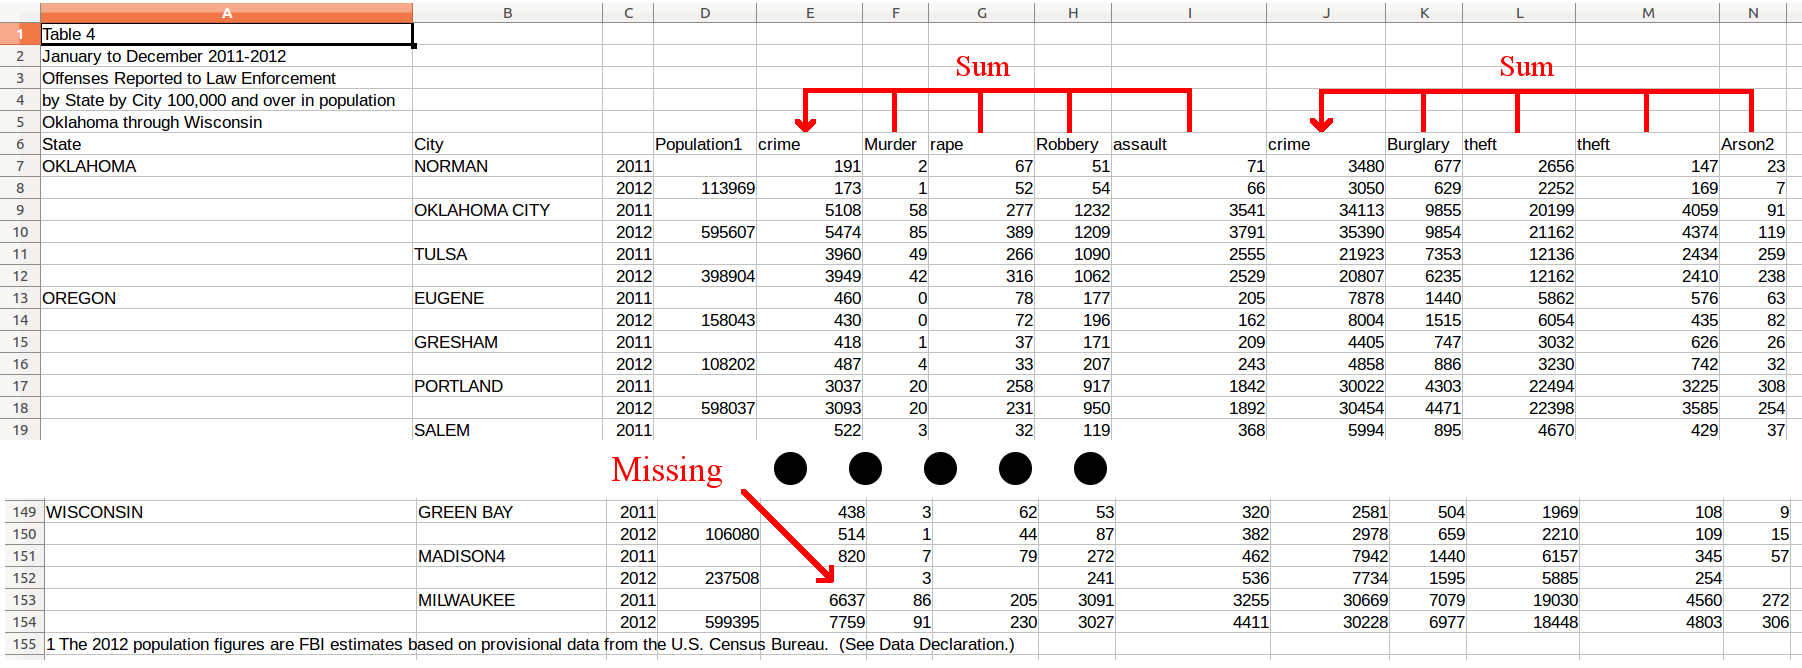
\includegraphics[width=0.85\textwidth]{figures/fbi_figure_highlighted.png}
  \end{center}
  \caption{Real world tabular constraint reconstruction: FBI crime statistics}
  \label{fig:fbi}
\end{figure*}


\sergey{I think there should be three things: key example evaluated, benchmark of 30 spreadsheets and maybe the FBI example, how we can detect interesting dependencies and correct potential mistakes}


{\bfseries
  Experimental questions
}

\begin{itemize}
  \item  How accurate are we? (Accuracy / recall)
  \item  How fast are we and which factors affect the runtime (how)?
  \item  How general is our approach, what limitations are there?
\end{itemize}


\section{Related Work}
\sergey{key bullet points for Luc and possibly Samuel and me to make related work section}

\sergey{ECAI reference style file ignores their guideline and their guideline ignores what is written in the guidelines!}
flashfill, flashextract, flashmeta \cite{flashfill,flashextract,flashmeta}
\begin{itemize}
  \item their supervised vs our unsupervised approach
  \item they look for a single ``smallest'' solution, we enumerate them all
  \item they are looking for a function, we solve constraint satisfaction problems
  \item we do not assume classic row based data layout, we work in the tabular setting
\end{itemize}

sketch \cite{sketch}
\begin{itemize}
  \item look for a constant that would fill in the gap in a program
  \item tailored for programming languages
  \item similar to model checking
  \item looks for a single solution
  \item similar to constraint satisfaction and sat, where one is interested in a single assignment that works for any potential input
\end{itemize}

tabular \cite{tabular}
\begin{itemize}
  \item language based on the excel tables that specify probabilistic models
  \item a system for probabilistic inference and similarity mostly in the usage of excel
  \item probabilistic constraint satisfaction (?) and graphical models
  \item single solution again
\end{itemize}

modelseeker \cite{modelseeker} \sergey{Samuel, Luc, probably you would need elaborate here more in details}

\begin{itemize}
  \item not designed for excel-like data representation (type consistency, groups, etc)
  \item not designed for excel-like constraints (lookups, conditional ifs, etc)
  \item does not support user extensions (?)
\end{itemize}

claudien \cite{claudien} \sergey{Samuel, Luc, you would need to help with this one}

\section{Discussion and Conclusions}
\sergey{link to the github with implementations and the dataset}


\sergey{Future version, extensions, declarative stuff, bla-bla here}
discussion: what would be a language to extend the system, what would be the user interface? can it be used by community?  can it be complitely automated? interaction with user and highlighing?


conclusions 
points: 1) can be a base for an actual plugin or a function in excel 2) novel problem and challenge for systems and constraint solvers 3) can be part of the complicated pipeline togehter with the header detection



\bibliographystyle{ecai}
\bibliography{references}
\end{document}
%%%%%%%%%%%%%%%%%%%%%%%%%%%%%%%%%%%%%%%%%%%%%%%%%%%%%%%%%%%%%%%%%%%%%%
